%% LyX 2.4.4 created this file.  For more info, see https://www.lyx.org/.
%% Do not edit unless you really know what you are doing.
\documentclass[english,brazil]{article}
\PassOptionsToPackage{natbib=true}{biblatex}
\usepackage[T1]{fontenc}
\usepackage{textcomp}
\usepackage[utf8]{inputenc}
\usepackage{babel}
\usepackage{float}
\usepackage{url}
\usepackage{graphicx}
\usepackage[bookmarks=true,bookmarksnumbered=false,bookmarksopen=true,bookmarksopenlevel=1,
 breaklinks=false,pdfborder={0 0 0},pdfborderstyle={},backref=false,colorlinks=false]
 {hyperref}
\hypersetup{pdftitle={Uma proposta metodológica que articula a resolução literal de problemas de Física e o software MathJSLab},
 pdfauthor={Sergio Lindau},
 pdfkeywords={Pensamento Computacional. Resolução Literal de Problemas. Ensino de Física. MATLAB.}}

\makeatletter

%%%%%%%%%%%%%%%%%%%%%%%%%%%%%% LyX specific LaTeX commands.
%% Because html converters don't know tabularnewline
\providecommand{\tabularnewline}{\\}

\makeatother

\usepackage[style=authoryear-comp]{biblatex}
\addbibresource{mathjslab.bib}
\begin{document}
\title{Uma proposta metodológica que articula a resolução literal de problemas
de Física e o software MathJSLab}
\author{Sergio Lindau\\
\href{mailto:sergiolindau@gmail.com}{sergiolindau@gmail.com}\\
\href{https://orcid.org/0009-0006-9115-0291}{ORCID: 0009-0006-9115-0291}}
\date{13 de maio de 2026}
\maketitle
\begin{abstract}
Este trabalho propõe que o aprendizado de Física e Matemática no Ensino
Médio oriente-se pela resolução literal de problemas, delegando a
execução numérica a ferramentas computacionais. Para viabilizar esta
proposta, apresentamos o MathJSLab, software de licença livre, que
simula um subconjunto da linguagem MATLAB. A metodologia proposta
é sustentada por uma fundamentação epistemológica, ontológica e semiótica,
amparada na Teoria Ator-Rede e na Teoria da Atividade Histórico-Cultural.
Tais referenciais estruturam a base para os pilares do Pensamento
Computacional de maneira a superar suas críticas, culminando em uma
abordagem metodológica exemplificada e articulada a um recurso didático.
O estudo conclui fornecendo uma estratégia fundamentada para superar
as abordagens tradicionais centradas em cálculos manuais, integrando
efetivamente a matemática computacional ao cotidiano escolar.
\end{abstract}
\textbf{Palavras-chave:} Pensamento Computacional. Resolução Literal
de Problemas. Ensino de Física. MATLAB.
\selectlanguage{english}%
\begin{abstract}
This work proposes that the learning of Physics and Mathematics in
High School should be guided by the symbolic resolution of problems,
delegating numerical execution to computational tools. To make this
proposal viable, we present MathJSLab, a free software that simulates
a subset of the MATLAB language. The proposed methodology is supported
by an epistemological, ontological, and semiotic foundation, based
on Actor-Network Theory and Cultural-Historical Activity Theory. These
frameworks structure the basis for the pillars of Computational Thinking
in order to overcome its criticisms, culminating in a methodological
approach exemplified and articulated with a didactic resource. The
study concludes by providing a well-founded strategy to overcome traditional
approaches centered on manual calculations, effectively integrating
computational mathematics into the daily life of High School education.
\end{abstract}
\textbf{Keywords:} Computational Thinking. Symbolic Problem Solving.
Physics Teaching. MATLAB.
\selectlanguage{brazil}%

\section{INTRODUÇÃO}

A resolução literal (ou simbólica) de problemas consiste em enumerar
todas as equações pertinentes para a solução e realizar manipulações
algébricas com variáveis simbólicas antes de substituir os valores
numéricos, converter unidades e fazer o cálculo aritmético, obtendo
a solução numérica particular do problema.

Na literatura de Ensino de Física, esse método é descrito como forma
de promover uma resolução significativa, em oposição à abordagem mecânica
para solucionar o problema. Isso também significa que os estudantes,
ao solucionarem um problema dessa maneira, elaboram as representações
algébricas e simbólicas de situações físicas reais, recriando os processos
de modelagem e dedução que caracterizam a atividade científica. Em
geral, a resolução de problemas pode ser compreendida como uma estratégia
que mobiliza conhecimentos prévios e desenvolve o raciocínio lógico
(\citealp{karam2009habilidades,oliveira2017problemas}). Outra motivação
para empreender uma metodologia baseada na resolução literal de problemas
justifica-se pela recorrente dificuldade que observamos nos alunos
ao aplicar suas competências matemáticas já consolidadas no domínio
da física. Pesquisas indicam que as falhas ocorrem não por deficiência
em matemática abstrata, mas pela incapacidade de contextualização
(\citealp{badmus2024physics,ince2018overview}). Na física, equações
descrevem sistemas reais e símbolos carregam significados físicos
específicos, diferindo das relações puramente abstratas da matemática.
Pesquisas de mais de 30 anos atrás (\citealp{perez1992questionando})
já apontavam a tendência de transformar a resolução de problemas,
em geral, em um operativismo mecânico e superficial. Portanto, o desafio
pedagógico central no ensino de física reside na tradução e aplicação
do conhecimento matemático nos modelos dos fenômenos físicos. Além
disso, é reconhecido que a resolução de problemas, em geral, é uma
competência essencial para o século XXI e que se trata de uma habilidade
cognitiva de alto nível (\citealp{ince2018overview}).

Na atualidade, o termo \textit{Resolução Literal de Problemas} tornou-se
uma expressão demasiado pesada, e muitas de suas formulações originais
foram integradas ao escopo do \textit{Pensamento Computacional} (PC).
Este é definido como um método cognitivo para solucionar problemas
complexos de maneira que tanto humanos quanto máquinas possam executá-los
efetivamente (\citealp{wing2006computational}). O PC também pode
ser definido de diversas outras formas, mas sempre é feita uma diferenciação
crítica: enquanto a computação é o processo definido em termos de
um modelo subjacente (a linguagem, algoritmos, estruturas de dados,
a máquina, etc.). O PC é o processo mental para formular o problema
e derivar as soluções que esse processo executará. Ou seja, não se
trata apenas de programar, mas de usar uma capacidade analítica para
elaborar abstrações matemáticas e estruturar problemas de modo que
técnicas de design de algoritmos e resolução de problemas possam ser
aplicadas eficazmente (\citealp{aho2011computational}).

O PC está integrado ao sistema educacional nacional na forma de um
dos eixos estruturantes do complemento à BNCC -- Computação (\citealp{brasil2022bncc}),
com os eixos de \textsl{Mundo Digital} e \textsl{Cultura Digital}.

O que propomos é que os estudantes, durante a solução literal de problemas,
realizem outra prática comum da atividade científica atual: delegar
a computação numérica do problema a uma ferramenta de matemática computacional.
Assim, essa metodologia didática que propomos está alinhada epistemológica
e ontologicamente à prática científica contemporânea: torna a atividade
didática em ação e, uma ação análoga aos agenciamentos da Ciência
e Engenharia modernas.

Essa separação entre o trabalho simbólico e dedutivo (feito à mão)
e o trabalho numérico e executável (feito via código) permite deslocar
o foco pedagógico para o desenvolvimento de competências mais profundas:
a capacidade de modelar, representar, deduzir, abstrair e traduzir
o mundo físico em linguagens simbólicas.

Para tornar nossa proposta metodológica plenamente viável e mantê-la
viável a longo prazo, passível de ser utilizada por professores na
atividade didática cotidiana, bem como servir de base para pesquisas
científicas na área de educação, desenvolvemos o software MathJSLab
(\citealp{lindau2026mathjslab}), que simula um subconjunto da linguagem
MATLAB, sendo executado no ambiente do navegador.

Adicionalmente, damos início à elaboração de uma síntese teórica fundamentada
na Teoria Ator-Rede (TAR) (\citealp{latour2012reagregando}) e na
Teoria da Atividade Histórico-Cultural (TAHC) (\citealp{vygotsky2007social,leontiev2022atividade,cenci2018atividade}),
cuja convergência justifica-se pela centralidade do conceito de mediação
em ambos os quadros. Embora o Pensamento Computacional (PC) ofereça
um arcabouço instrumental e sistematizado para a ação didática, a
adoção desses referenciais mais amplos provê a fundamentação epistemológica,
ontológica e semiótica necessária para estabelecer diretrizes pedagógicas
claras e justificar a proposta integral deste trabalho. Sob essa perspectiva
integrada, pretendemos superar as críticas recorrentes ao PC e ao
ensino focado na resolução de problemas, consolidando um quadro teórico
que sustente a metodologia de ensino de física baseada na resolução
literal de problemas, na qual a execução de cálculos manuais é delegada
a ferramentas de matemática computacional.

A síntese entre a TAR e a TAHC caracteriza o MATLAB como um actante
de múltiplos agenciamentos epistemológicos e ontológicos na rede sociotécnica
da matemática. Como mediador ativo, o software reconfigurou a atividade
humana e a cognição coletiva, expandindo o escopo de problemas tratáveis
e estabilizando novas práticas científicas. Esta fundamentação permite
superar críticas conceituais ao Pensamento Computacional, orientando
ações didáticas para o ensino de Física.

O objetivo deste trabalho é apresentar o MathJSLab como recurso didático
para a resolução literal de problemas. A pesquisa justifica-se pelo
interesse na transição da ênfase pedagógica: em vez do tradicional
cálculo numérico manual, propõe-se desenvolver competências em codificação
da solução numérica a partir da solução simbólica. Ao delegar a componente
aritmética à ferramenta computacional, a proposta integra a matemática
à realidade da pesquisa contemporânea, que delega a ferramentas computacionais
a execução numérica dos modelos, priorizando a inteligibilidade dos
fenômenos físicos.

\section{DESENVOLVIMENTO}

Este trabalho ancora-se em duas diretrizes axiomáticas do construtivismo,
fundamentadas na epistemologia genética e na teoria do desenvolvimento
histórico-cultural, para estruturar uma metodologia didática no âmbito
do construcionismo.

O primeiro axioma estabelece que a aprendizagem deve promover a recomposição
da filogênese na ontogênese do indivíduo. Sob essa premissa, os processos
didáticos são desenhados para o aprendiz reproduzir, de forma análoga
e mediante transposições didáticas, o percurso histórico de produção
do conhecimento científico do coletivo humano. Alinhada ao pensamento
de \citet{piaget2010simbolo}, \citet{bruner2000instrucao}e \citet{vygotsky2007social},
essa diretriz orienta uma pedagogia baseada na imitação, reconstrução
e recomposição das práticas e conceitos em sua gênese histórica e
lógica.

O segundo axioma fundamenta-se na tese de Vygotsky sobre a internalização
de mediações culturais. O desenvolvimento cognitivo é compreendido
como um processo mediado por sistemas de signos e ferramentas (como
a linguagem, a escrita e a matemática) que, ao serem incorporados
e reconstruídos internamente, transmutam funções psicológicas elementares
em funções psicológicas superiores. Tais mediadores não são meros
canais comunicativos, mas instrumentos que reorganizam o pensamento
e expandem a capacidade intelectual por meio da interação social e
da instrução na Zona de Desenvolvimento Proximal (ZDP). A apropriação
bem-sucedida dessas mediações e o consequente desenvolvimento autônomo
manifestam-se na habilidade do estudante em articular e transitar
entre diferentes sistemas de representação equivalentes (verbal, simbólico
e gráfico, por exemplo).

Com base nesses princípios axiomáticos, propomos uma articulação teórico-metodológica
entre a Teoria Ator-Rede (TAR) e a Teoria da Atividade Histórico-Cultural
(TAHC). O objetivo é fornecer um arcabouço conceitual robusto para
o planejamento e análise de práticas educativas no ensino de Física,
Matemática e Computação, focando especificamente na \textsl{Resolução
Literal de Problemas}. Essa abordagem visa integrar a modelagem simbólica
e o uso de ferramentas computacionais como actantes e mediadores essenciais
para a inteligibilidade dos fenômenos científicos contemporâneos.

A TAHC afirma que a aprendizagem e o desenvolvimento cognitivo de
uma pessoa são fundamentalmente moldados pelas interações sociais
e pela cultura que a cerca, assim como o coletivo humano é moldado
pelas mediações na interação social e no processo cultural. A TAR
enfatiza a agência dos atores não humanos, estabelecendo redes sociotécnicas
estáveis. Um amálgama entre as duas teorias para tratar de assuntos
da Epistemologia das Ciências ou mesmo da Educação, ou ainda de Teorias
Cognitivas, parece não somente viável, mas bastante adequado. A convergência
entre TAR e TAHC centra-se na premissa de que a ação e interação humana
são sempre processadas por elementos intermediários. Entretanto, as
teorias operam em escalas e objetivos distintos: a mediação (TAHC)
refere-se ao desenvolvimento de funções psicológicas superiores (interiorização)
e a tradução (TAR) trata da estabilização de redes sociotécnicas e
coletivos (exteriores à subjetividade).

O Pensamento Computacional (PC) consolidou-se como uma competência
central do século XXI, extrapolando a ciência da computação e assumindo
relevância geral na resolução de problemas em múltiplos domínios.
Suas bases históricas remontam à década de 1950, embora muitas de
suas ideias fundamentais sejam significativamente mais antigas. O
termo foi formalmente empregado por Seymour Papert em 1980 (\citet{papert1993mindstorms})
e depois em 1996. Tais conceitos apoiam-se em trabalhos desenvolvidos
pelo autor em conjunto com Cynthia Solomon no artigo “Twenty things
to do with a computer” em 1971 (\citealp{papert1972twenty}). Antes
da popularização do termo, noções correlatas já circulavam sob outras
denominações (\citealp{tedre2016quest}). A noção ganhou projeção
global no campo educacional em 2006, a partir de um trabalho de Jeannette
Wing (\citealp{wing2006computational}), que definiu o PC como uma
habilidade básica universal, defendendo que ele deve ser integrado
à educação de todas as crianças de forma análoga à leitura, à escrita
e à aritmética.

Apesar de amplamente aceito, o pensamento computacional (PC) é alvo
de críticas quanto à sua imprecisão conceitual e à dificuldade de
distingui-lo de outras formas de raciocínio lógico, científico ou
de engenharia (\citealp{tedre2016quest,jones2016trouble}). Existe
também a crítica sobre a inclinação de forçar soluções computacionais
em contextos inadequados ou campos alheios (\citealp{tedre2016quest}).
Aponta-se ainda que a ênfase excessiva na resolução técnica e algorítmica
de problemas pode obscurecer as implicações sociais, éticas e ambientais
inerentes às tecnologias criadas (\citealp{easterbrook2014systems,tedre2016quest}).
Soma-se a isso o debate sobre a melhor estratégia de inserção curricular:
enquanto alguns defendem a integração transversal em disciplinas como
Matemática e Ciências (\citealp{barr2011bringing,grover2013review}),
outros argumentam que o PC deve ser ensinado como uma disciplina autônoma
e distinta (\citealp{wolfram2010code}). Os pesquisadores também destacam
as limitações da generalização de modelos educacionais e pesquisas
predominantemente formulados nos Estados Unidos e na Europa, questionando
sua eficácia e adequação quando transpostos para outros contextos
culturais (\citealp{saqr2021scientometric,tedre2016quest}).

O PC é comumente expresso por quatro pilares fundamentais que, sob
estes referenciais integrados, deixam de ser técnicas isoladas, sendo
compreendidos como funções psicológicas superiores resultantes da
apropriação de artefatos históricos:
\begin{enumerate}
\item \textit{Decomposição de tarefas}: equivale à \textit{despontualização}\footnote{A \textit{pontualização}, na ótica da TAR, refere-se ao processo pelo
qual uma rede complexa e heterogênea de elementos (humanos e não-humanos:
técnicas, pessoas, instituições, documentos) é “reunida” ou “traduzida”
para agir em conjunto, como se fosse um único agente ou uma entidade
simples: para fins de análise, um único ponto ou “atores-rede”. Quando
uma rede funciona bem e é pontualizada, seus componentes internos
se tornam invisíveis. Um computador, por exemplo, é uma rede pontualizada
(chips, fios, eletricidade, software, usuários) que tratamos simplesmente
como “o computador”, tornando-se uma “caixa-preta”. A pontualização
nunca é permanente. Ela precisa ser constantemente mantida, caso contrário,
a rede se desfaz (\textit{despontualização}) e a caixa-preta “se abre”.}(a abertura de “caixas-pretas”) para rastrear actantes (TAR) e à internalização
da divisão do trabalho coletivo (TAHC).
\item \textit{Reconhecimento de Padrões}: identificação de inscrições imutáveis
(TAR) e signos culturais sedimentados que permitem antecipar comportamentos
da rede.
\item \textit{Abstração e Generalização}: processo de tradução para criar
um “ponto de passagem obrigatório” (TAR) e movimento em direção ao
conceito formal via ZDP (TAHC).
\item \textit{Algoritmos}: mediadores ativos que transformam significados
(TAR) e ferramentas intelectuais que reorganizam o pensamento do aprendiz
(TAHC).
\end{enumerate}
Essa fundamentação contorna críticas centrais ao PC. A imprecisão
conceitual é superada ao definir o PC como a construção de redes de
mediação voltadas à executabilidade por agentes. O chauvinismo computacional
é combatido pela Simetria Generalizada, que exige a relevância das
implicações sociais e éticas como partes da rede. Por fim, a crítica
à generalização de modelos ocidentais é respondida pela TAHC, que
enfatiza que todo desenvolvimento é histórica e culturalmente situado.

Uma vez que apenas um esboço dessa integração teórica entre a TAR
e a TAHC já dá conta de sustentar em sólida base os pilares do PC,
superando suas críticas principais, podemos passar a descrever, sem
a pretensão de esgotar o assunto, a matemática e o MATLAB sob a perspectiva
desse amálgama teórico. Assim, fazemos com a intenção de articular
e melhor exemplificar como as atividades didáticas que propomos, de
resolução literal de problemas usando o MathJSLab, podem ser pensadas
e executadas.

A compreensão contemporânea da matemática e de suas ferramentas computacionais
exige um olhar que transcenda a dicotomia entre o sujeito que pensa
e o objeto pensado. Sob as lentes da Teoria Ator-Rede (TAR) e da Teoria
da Atividade Histórico-Cultural (TAHC), a matemática e o código algorítmico
revelam-se inseparáveis dos sistemas de representação e dos meios
técnicos e culturais de cômputo que os sustentam. Estes não são meros
suportes ou ferramentas auxiliares, mas atores não-humanos ativos,
co-constituintes de uma rede sociotécnica vasta e heterogênea. A matemática,
pilar fundamental do desenvolvimento civilizatório, opera hoje como
uma infraestrutura invisível que sustenta desde complexas operações
financeiras até a produção científica de ponta, fruto de um processo
de tecedura histórica secular.

Não raros estudos sob a perspectiva da educação caracterizam a matemática
dessa forma, mesmo que não explicitando estes referenciais teóricos
que propomos:
\begin{quotation}
Dessa forma, a Matemática está arraigada nos conceitos físicos; por
exemplo, ela está encarnada na ciência com função mediadora e não
constitui um anexo, um adendo. Assim, é possível afirmar que a Matemática
como instrumento formal e técnico pode ser compreendida em outros
contextos, entretanto essa Matemática como habilidade estruturante
da Física não pode ser compreendida e aplicada independentemente (\citealp{pietrocola2002matematica}
apud \citealp{oliveirajunior2021matematica}, p. 2).
\end{quotation}
Na perspectiva da TAR, a matemática é uma rede complexa onde a agência
é distribuída entre humanos e não-humanos: escribas, papiros e tábuas
de argila, numerais, engenheiros, ábacos, astrolábios, construtores,
notações, cientistas, axiomas, algoritmos, instrumentos, equações,
teoremas, comerciantes, navegadores, astrônomos, contadores, pesos
e medidas, comitês de padronizações, economistas, currículos, instituições
de ensino e pesquisa, professores, manuais didáticos, alunos, convenções
simbólicas, linguagens de programação, algoritmos, calculadoras de
engrenagens e processadores de chips de silício, entre uma infinidade
de outros agentes agregados num coletivo inteiriço povoado de sujeitos
e objetos. Esta rede não se limita a objetos materiais; muitos de
seus actantes mais poderosos são simbólicos, como axiomas, teoremas
e convenções notacionais. A prática matemática só se concretiza por
meio de formas eficazes de registrar e manipular relações e padrões
de maneira consensual. Isso faz com que as suas aplicações da matemática
ao longo do processo histórico sempre fiquem bem registradas e, quando
começou a ser aplicada na área da ciência, passou a ser mais bem documentada,
de maneira absolutamente formal (\citealp{badmus2024physics}).

Tais registros, contudo, não são neutros. Eles constituem inscrições
(materiais ou simbólicas) que reconfiguram os problemas passíveis
de análise, estabilizam práticas e reorganizam a própria cognição
humana, pois parte desses registros são mediadores culturais, conforme
a TAHC estabelece, que acabam por ser internalizados, dando origem
a funções psicológicas superiores. Ou seja: tais inscrições tornam-se
agentes ontológicos e epistemológicos.

Sob o olhar da TAHC, essas inscrições atuam como ferramentas psicológicas
e signos que medeiam a atividade humana. Enquanto o texto escrito
transporta significados por um canal unidimensional e fonético, as
representações matemáticas operam em estruturas multidimensionais
com aspectos instrumentais e operativos ilimitados. O caminhar para
abstrações crescentes não é um exercício de distanciamento da realidade,
mas uma estratégia para aglutinar actantes de poder e garantir um
alcance consensual e absoluto sobre o mundo real. A estabilização
desta rede depende intrinsecamente das instituições de educação formal,
onde currículos e pedagogias formatam modos de pensar coletivos, consolidando
o “saber-fazer” de maneira cumulativa através das gerações.

O software MATLAB (Matrix Laboratory) exemplifica a materialização
desse caráter instrumental e operativo do código algorítmico, emergindo
como um actante epistemológico. Apresentado comercialmente como uma
plataforma otimizada para a resolução de problemas científicos e de
engenharia. Sua linguagem baseada em matrizes é descrita como a “maneira
mais natural” de expressar a matemática computacional (\citealp{mathworks2025product}).
Contudo, para além de sua definição técnica como um interpretador
multiparadigma, o MATLAB deve ser compreendido como um agente ontológico
e epistemológico. Ele intervém na constituição do real ao definir
o que pode ser calculado e mediado, agindo como um nó central que
traduz o saber algorítmico em ação concreta.

A origem do MATLAB não reside em um estalo isolado de genialidade,
mas é o resultado de uma densa série de inscrições prévias e associações
heterogêneas. Suas raízes remontam aos trabalhos de J. H. Wilkinson
e outros pesquisadores nas décadas de 1960 e 1970, cujos algoritmos
para autovalores e equações lineares foram traduzidos num manual didático
(\citealp{wilkinson1971handbook}) e em bibliotecas Fortran como EISPACK
e LINPACK\footnote{O EISPACK e o LINPACK são bibliotecas Fortran para álgebra linear
desenvolvidas no \textit{Argonne National Laboratory}: a EISPACK foca
no cálculo de autovalores e autovetores, enquanto a LINPACK resolve
equações lineares e problemas de mínimos quadrados. Ambas foram sucedidas
pelo LAPACK. Disponíveis em:\url{ https://www.netlib.org/eispack/},
\url{https://www.netlib.org/linpack/} e \url{https://www.netlib.org/lapack/}.} no \textit{Argonne National Laboratory} (\citealp{haigh2008moler,moler2004origins,moler2018brief,moler2020history}).
Nestes termos, o MATLAB emerge de uma aglutinação de atores humanos
que produziram equações e artigos, os quais foram posteriormente condensados
em manuais e bibliotecas que se tornaram, em si mesmos, protagonistas
da rede ao serem traduzidos em código executável. O nascimento do
primeiro MATLAB, codificado por Cleve Moler em 1976 na Universidade
do Novo México (\citealp{haigh2008moler}), foi um ato de tradução.
Moler, um dos desenvolvedores da biblioteca LINPACK, lecionando a
disciplina de Álgebra Linear e Análise Numérica na Universidade do
Novo México, buscou criar uma maneira de seus alunos poderem usar
os recursos das bibliotecas EISPACK e LINPACK sem que fosse necessário
escrever códigos em linguagem de programação, tendo que rodar todo
o ciclo de montagem de um programa: edição, compilação, carregamento
e execução. O MATLAB original era, portanto, um mediador que simplificava
a interação entre o estudante (sujeito) e a álgebra linear computacional
(objeto/atividade). Desde então, passou a agir mediando, traduzindo
e estabilizando inscrições na rede sociotécnica da matemática.

Ao longo dos anos 1980, a união de Moler com John Little e Steve Bangert
para reprogramar o software em C e lançá-lo comercialmente pela MathWorks
em 1984, marcou um processo de pontualização. O software deixou de
ser uma ferramenta acadêmica gratuita para se tornar uma “caixa-preta”
estável, uma ferramenta-padrão de engenharia reconhecida mundialmente.
Seu logotipo, o gráfico de um problema de autovalor de uma membrana
em forma de L, funciona como um signo que referencia as origens memoráveis
e a rede de algoritmos de Wilkinson e Forsythe que o precederam.

A integração da matemática e do MATLAB sob os referenciais da TAR
e da TAHC revela que a inteligência e a capacidade de resolução de
problemas não residem apenas no cérebro humano, mas no desempenho
da rede sociotécnica. As aplicações do MATLAB abarcam os campos dos
“sistemas de segurança ativa para automóveis, espaçonaves interplanetárias,
dispositivos de monitoramento de saúde, redes elétricas inteligentes
e redes celulares de evolução de longo prazo, aprendizado de máquina,
processamento de sinais, processamento de imagens, visão computacional,
comunicações, finanças computacionais, projetos de controle e robótica”
(\citealp{mathworks2025product}). Por isso, o MATLAB não pode ser
considerado apenas um instrumento; ele é um actante que induz novas
formas de agência. Ele reorganiza a atividade humana ao permitir que
operações de álgebra linear sejam aplicadas a matrizes multidimensionais
intuitivamente, atuando como um agente eficaz que executa instruções
e materializa o pensamento computacional.

Nesse cenário, a matemática e o software são mediadores que moldam
a percepção do mundo. A estabilidade desses actantes é garantida pela
sua inscrição contínua em currículos e na prática profissional, onde
humanos e não-humanos interagem em simetria generalizada. O amálgama
destas teorias permite reconhecer que, ao utilizarmos o MATLAB, estamos
nos associando a séculos de história matemática, bibliotecas de código
estabilizadas e instituições de ensino, formando um coletivo onde
o saber, o fazer e o saber-fazer são distribuídos e performados continuamente
para moldar e compreender a realidade, estabelecendo cada vez mais
uma simetria entre o humano e o algoritmo.

\subsection{O MATHJSLAB}

O MathJSLab foi desenvolvido inicialmente na linguagem JavaScript\footnote{JavaScript implementa o padrão ECMAScript (nome da linguagem padronizada
pela ECMA-262), definindo sua sintaxe e tipos básicos, adicionando
APIs de ambiente (DOM no navegador, sistema de arquivos no Node.js);
Especificação: \url{https://262.ecma-international.org/16.0/index.html}.}, depois evoluindo para a linguagem TypeScript\footnote{TypeScript é um superconjunto fortemente tipado da linguagem JavaScript
que compila para JavaScript. Especificação: https://www.typescriptlang.org/.}. A meta de desenvolvimento inicial era criar uma calculadora que
permitisse definir variáveis e calcular expressões matemáticas com
as variáveis definidas. Assim poderia ser incorporado numa página
Web. As primeiras versões consistiam somente em substituição de caracteres
numa string (a expressão matemática de entrada) e a execução da função
\texttt{eval}\footnote{A função \texttt{eval} executa uma string com comandos JavaScript,
seguindo o conceito de \textit{bootstrap}: uma função que executa
comandos da própria linguagem.} sobre a string resultante. Não havia um mecanismo de interpretação
da string representando a expressão de entrada nem uma exibição adequada,
em notação matemática, da entrada e do resultado calculado.

Atualmente, o MathJSLab usa o ANTLR\footnote{ANTLR é um gerador de analisadores sintáticos que, a partir da especificação
de uma gramática, produz parsers para leitura, processamento ou tradução
de texto/bits. Disponível em \url{https://www.antlr.org/}.} para gerar o analisador léxico e sintático do seu interpretador e
usa a linguagem MathML\footnote{MathML é uma linguagem de marcação para descrever notação matemática,
capturando sua estrutura e conteúdo, com o objetivo de permitir o
uso de matemática na World Wide Web. Especificação: \url{https://www.w3.org/TR/mathml4/}.} para gerar expressões a serem em notação matemática usual. A ideia
inicial era fazer um software educativo que pudesse ser executado
no ambiente do navegador Web e pudesse treinar habilidades de codificação
de expressões matemáticas em linguagem de programação. Assim, a resolução
literal de problemas de física aparecia como a aplicação ideal para
a utilização do software e acrescentar habilidades de codificação
no âmbito do Ensino de Física. O nome, MathJSLab, é uma referência
à ideia de um laboratório matemático em JavaScript.

O software foi publicado de maneira planejada para ter plena disponibilidade,
possibilidade de desenvolvimento cooperativo, manutenção frequente,
ISBN atribuído e DOI definido para cada versão lançada. Assim, pode
ser referenciado adequadamente por qualquer trabalho de pesquisa que
o utilize como ferramenta de pesquisa ou objeto de estudo na área
da Educação. Além disso, ele é publicado com uma licença de software
livre permissiva, a licença MIT\footnote{A Licença MIT é uma licença de software de código aberto extremamente
permissiva e popular, originada no Instituto de Tecnologia de Massachusetts
(MIT). Ela permite que qualquer pessoa use, copie, modifique, distribua,
sublicencie e venda o software com poucas restrições, apenas mantendo
o aviso de direitos autorais original. Disponível em: \url{https://opensource.org/license/mit}}, e pode ser executado em qualquer dispositivo com conexão à Internet,
podendo ser instalado para ser utilizado offline também\footnote{Trata-se de uma aplicação Web Progressiva.}.
Todo o software foi desenvolvido com as mais modernas tecnologias
Web\footnote{HTML5, templates SCSS e Nunjucks, documentação em Markdown e Web Components.}
para garantir a máxima frequência de manutenção e possibilidades de
evolução futura. Toda a aplicação, bem como a documentação de ajuda
de cada comando, está traduzida em três idiomas: inglês, português
e espanhol. Toda a documentação foi escrita no formato Markdown\footnote{Markdown é uma linguagem de marcação leve para formatar texto simples
usando símbolos intuitivos e convertê-lo em HTML ou outros formatos.
Foi projetado para ser legível como texto puro e fácil de escrever,
sendo amplamente usado em documentação, sites e README de projetos.
Ver \url{https://www.markdownguide.org/}.}

\begin{figure}[H]
\begin{centering}
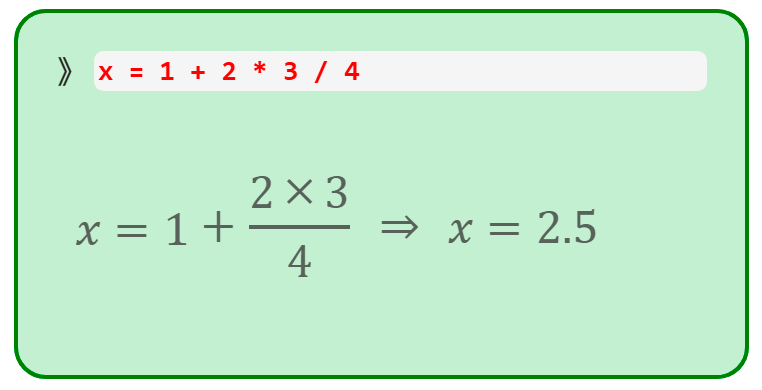
\includegraphics[scale=0.2]{mathjslab-prompt}
\par\end{centering}
\caption{Prompt de comando do MathJSLab, mostrando a tradução e solução do
código, exibindo em linguagem matemática usual.}\label{fig:mathjslab-prompt}

\end{figure}
.O prompt do MathJSLab, mostrado na Figura \ref{fig:mathjslab-prompt},
difere da forma como é o MATLAB por ser elaborado visando o segundo
axioma que adotamos, sobre a tradução de representações equivalentes.
O prompt recebe o comando em código e mostra logo abaixo a expressão
em notação matemática usual, como é costume adotar com papel e lápis.
Assim, o próprio observar o resultado de cada prompt já é um exercício,
treinando a tradução do código à notação matemática usual.

Para mostrar a resolução completa de um problema no ambiente do aplicativo,
mostramos uma sequência de prompts que resolvem a equação do 2º grau
pelo método de Bhaskara (Figura \ref{fig:mathjslab-bhaskara}). Cada
prompt digitado na forma de código é interpretado, computado e a entrada
e o resultado são exibidos em notação matemática usual.

\begin{figure}[H]
\begin{centering}
\begin{tabular}{ccc}
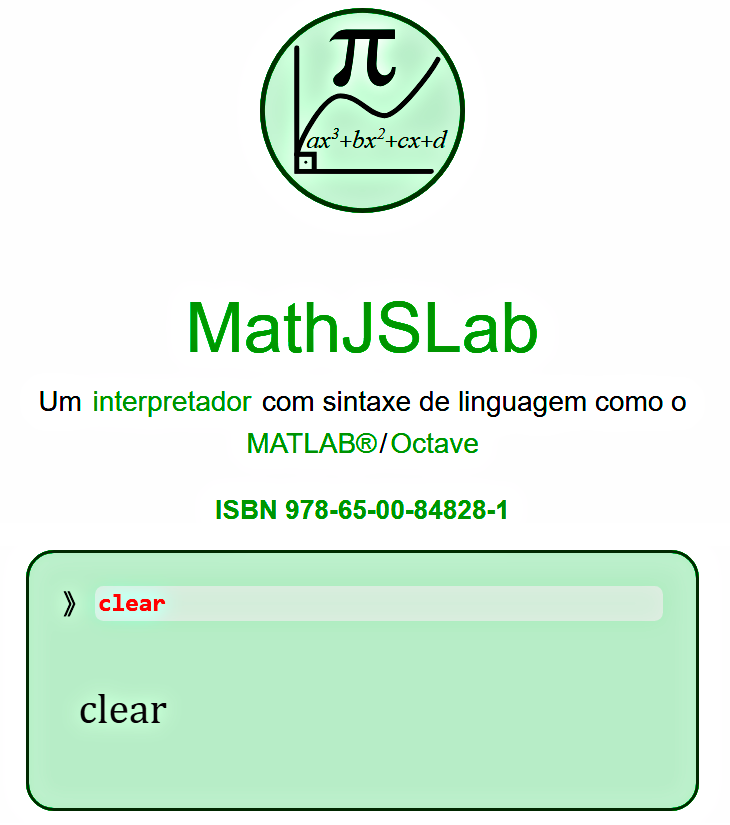
\includegraphics[scale=0.2]{mathjslab-bhaskara-1} &  & 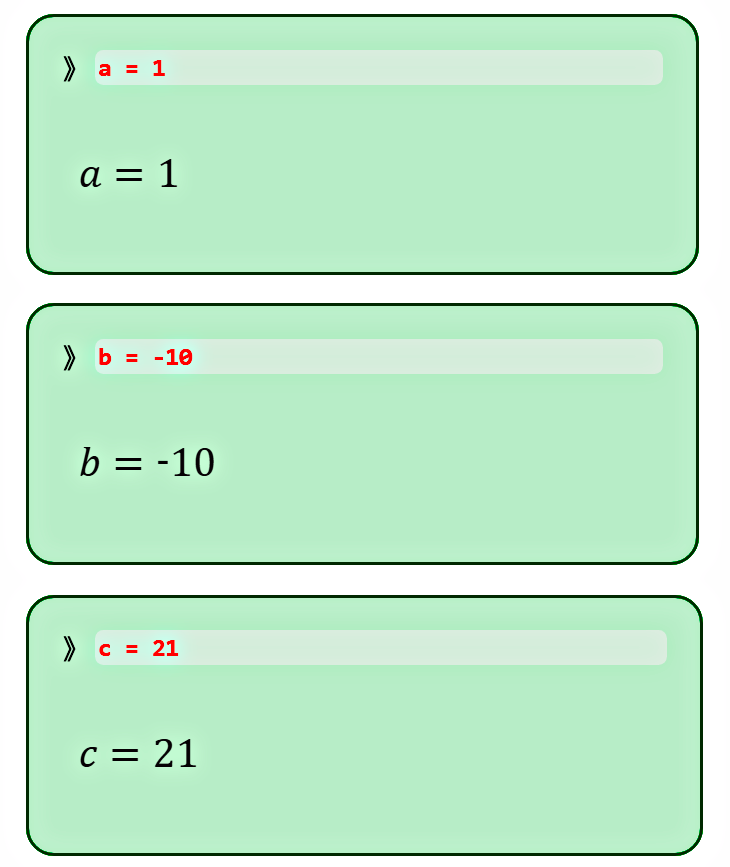
\includegraphics[scale=0.2]{mathjslab-bhaskara-2}\tabularnewline
(a) & $\longrightarrow$ & (b)\tabularnewline
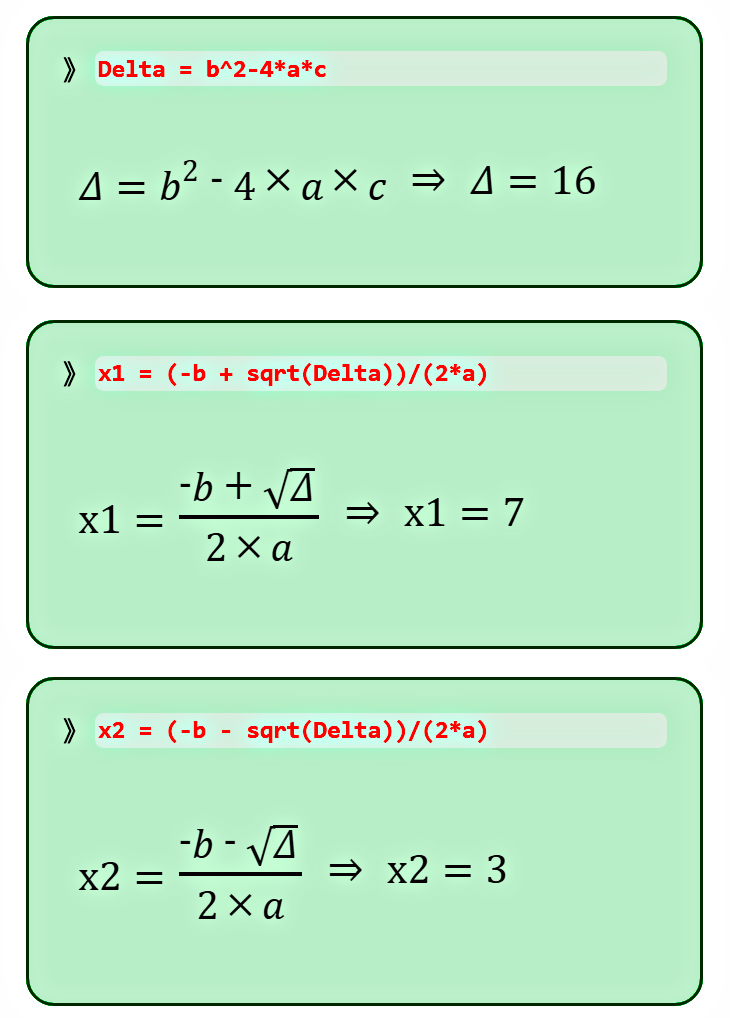
\includegraphics[scale=0.2]{mathjslab-bhaskara-3} &  & 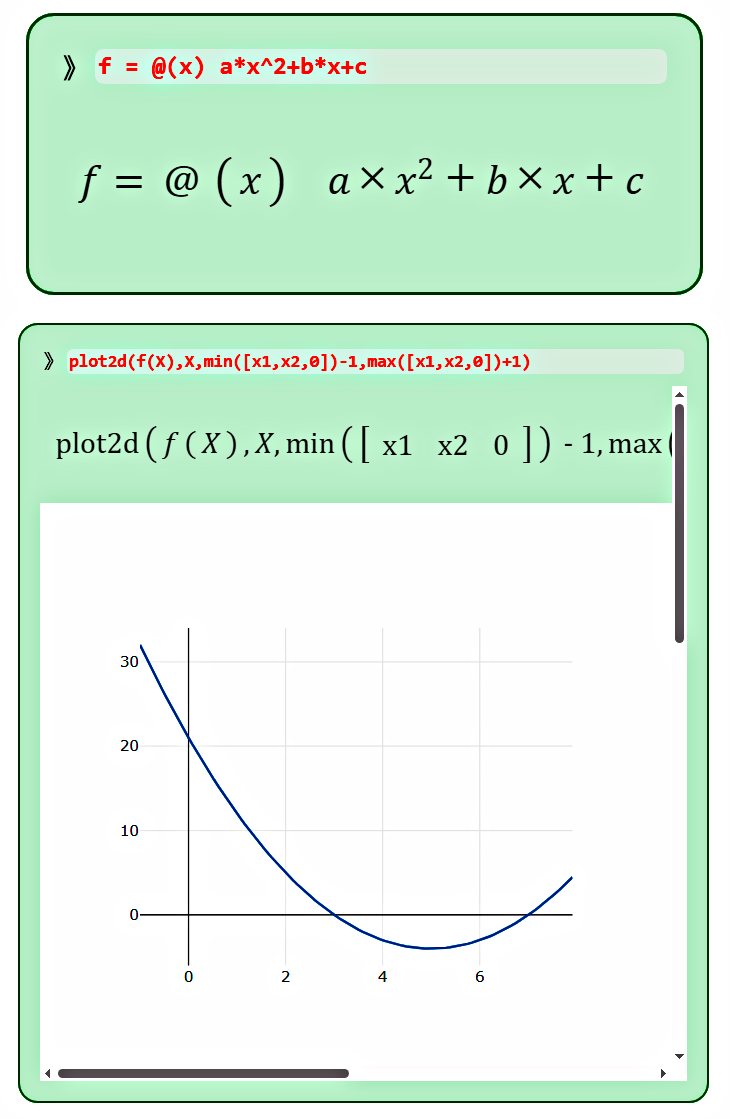
\includegraphics[scale=0.2]{mathjslab-bhaskara-4}\tabularnewline
(c) & $\longrightarrow$ & (d)\tabularnewline
\end{tabular}
\par\end{centering}
\caption{Telas do MathJSLab mostrando a resolução da equação do 2º grau: (a)
começa apagando todas as variáveis; (b) definição dos coeficientes
da equação; (c) solução pela fórmula de Bhaskara; (d) definição da
função e construção do gráfico.}\label{fig:mathjslab-bhaskara}
\end{figure}


\subsection{EXEMPLOS DE APLICAÇÃO DIDÁTICA EM NÍVEL DE ENSINO MÉDIO: RESOLUÇÃO
LITERAL DE PROLEMAS}

Para demonstrar atividades didáticas de resolução literal de problemas
no ensino de Física usando o MathJSLab, mostramos dois exemplos.

O primeiro exemplo é um problema do ENEM, onde é necessário solucionar
o problema num tempo minimamente viável e justifica-se por mostrar
toda a potencialidade dos métodos e recursos aqui apresentados.

O segundo exemplo é um problema análogo ao resolvido em experimentos
com plano inclinado. Este exemplo justifica-se pela relevância do
problema como actante e mediador cultural, e por exemplificar também
as transposições didáticas sem limites que podemos fazer quando os
objetos são pensados como actantes e mediadores socioculturais.

\subsubsection{UM PROBLEMA DO ENEM}

O Exame Nacional do Ensino Médio (ENEM), com grande número de questões
em cada caderno (90), tem tempo bastante limitado por questão para
executar sua solução. Questões que envolvem a manipulação de duas
ou mais equações exigem a resolução literal para que o tempo de solução
da questão seja minimamente viável. Um bom exemplo de questão assim
é a do ENEM de 2015, que está na Figura \ref{fig:enem-2015-carro-solar},
que trata de um carro movido por energia solar, calculando o tempo
que leva para atingir determinada velocidade.

A solução do problema consiste em equacionar a potência efetiva entregue
pelo painel solar em termos dos dados fornecidos e considerar que
essa energia é transformada em energia cinética, calculando o tempo
total através da definição de potência como a taxa de variação da
energia em relação ao tempo. Em resumo: a solução literal é o melhor
caminho.

O código para a solução da questão no MathJSLab está na Figura \ref{fig:codigo-enem-2015-carro-solar}.
É uma sequência de definições e cálculo de expressões baseada na resolução
literal do problema.

\begin{figure}[H]
\begin{centering}
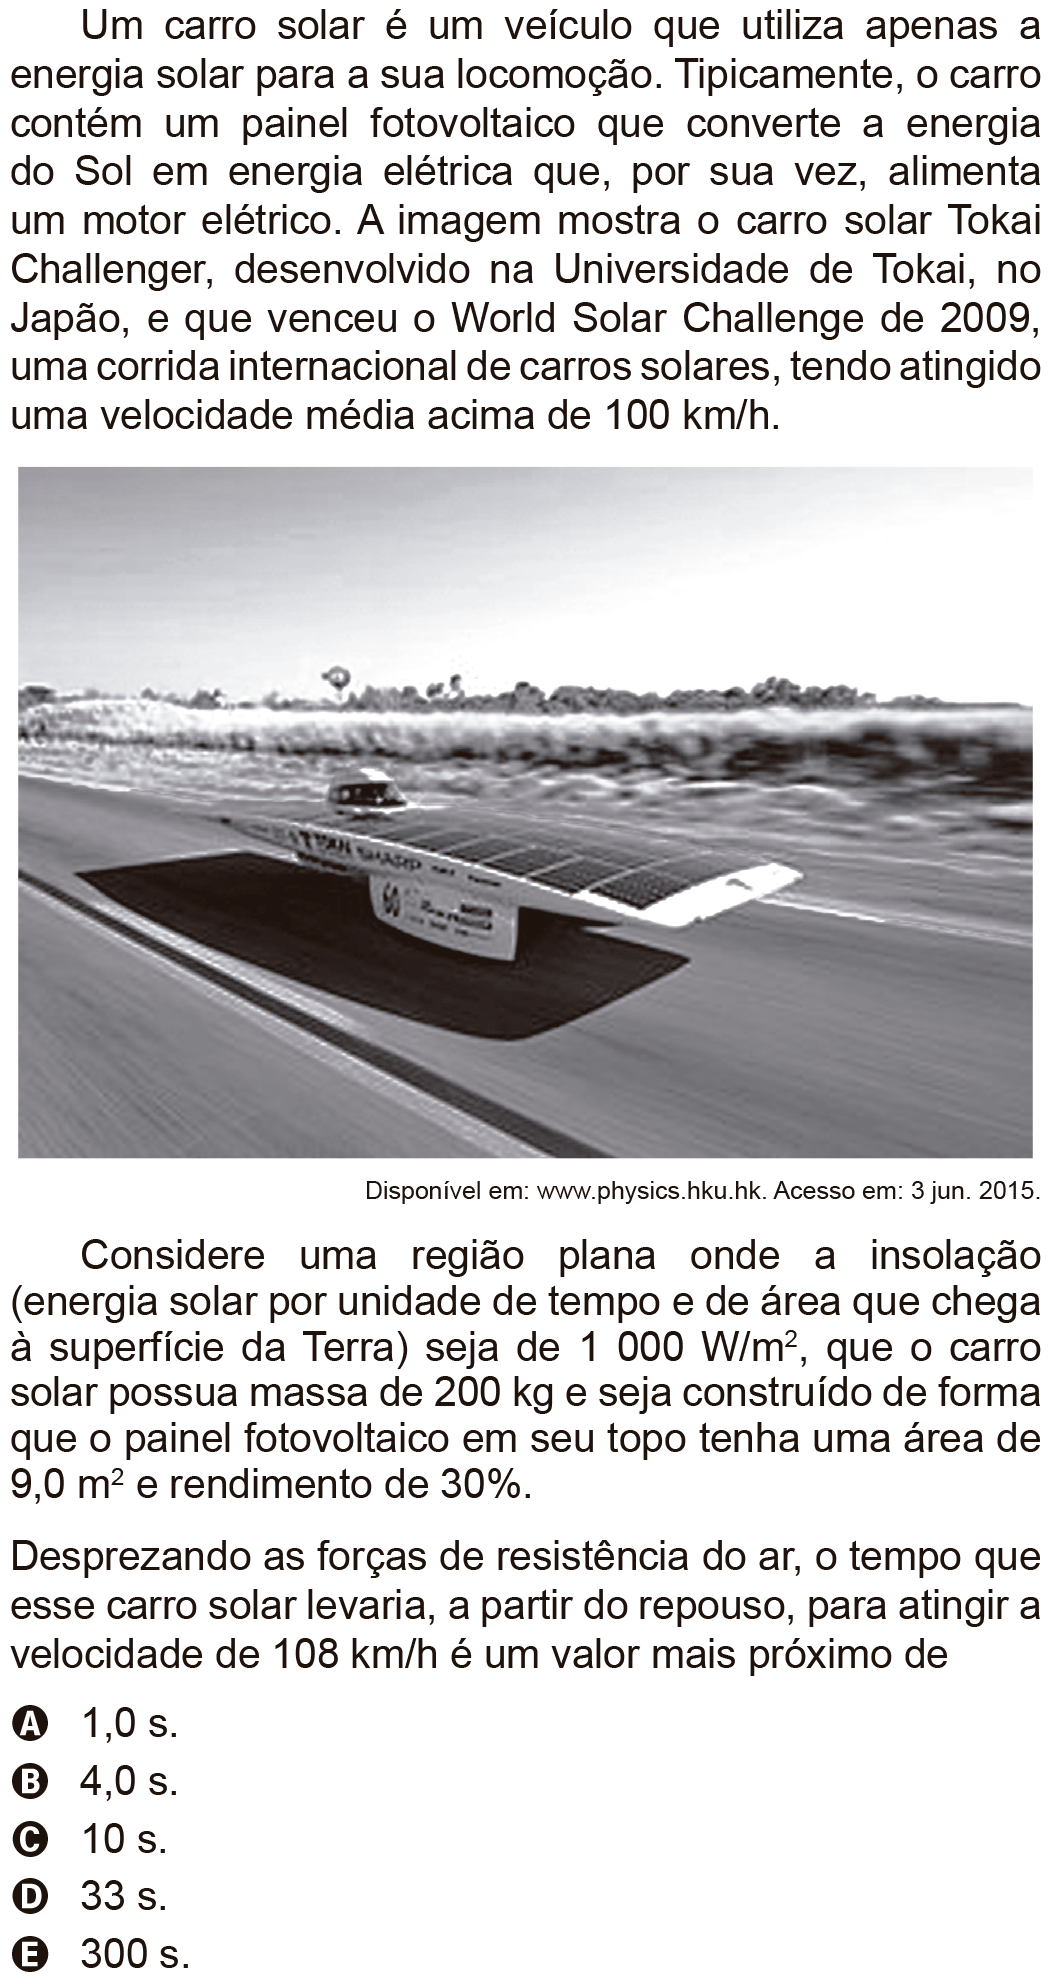
\includegraphics[scale=0.15]{enem-2015-carro-solar}
\par\end{centering}
\caption{Questão de física do ENEM 2015: desempenho de um carro solar.}\label{fig:enem-2015-carro-solar}
\end{figure}

\begin{figure}[H]
\begin{centering}
\begin{tabular}{ll}
\textbf{expressão} & \textbf{comentário}\tabularnewline
\texttt{\textbf{D\_P = 1000}} & \texttt{\textbf{\% densidade de potência da radiação solar}}\tabularnewline
\texttt{\textbf{m = 200}} & \texttt{\textbf{\% massa do carro}}\tabularnewline
\texttt{\textbf{A = 9}} & \texttt{\textbf{\% área do painel solar}}\tabularnewline
\texttt{\textbf{eta = 0.30}} & \texttt{\textbf{\% rendimento do painel solar}}\tabularnewline
\texttt{\textbf{Pe = D\_P {*} A {*} eta}} & \texttt{\textbf{\% potência efetiva do painel}}\tabularnewline
\texttt{\textbf{km = 1000}} & \texttt{\textbf{\% quilômetro em metros}}\tabularnewline
\texttt{\textbf{h = 60{*}60}} & \texttt{\textbf{\% hora em segundos}}\tabularnewline
\texttt{\textbf{m\_s = km/h}} & \texttt{\textbf{\% fator de conversão km/h em m/s}}\tabularnewline
\texttt{\textbf{v = 108 {*} m\_s}} & \texttt{\textbf{\% velocidade em m/s}}\tabularnewline
\texttt{\textbf{Ec = m {*} v\textasciicircum 2 / 2}} & \texttt{\textbf{\% energia cinética}}\tabularnewline
\texttt{\textbf{Delta\_t = Ec / Pe}} & \texttt{\textbf{\% tempo para adquirir a energia cinética}}\tabularnewline
\end{tabular}
\par\end{centering}
\caption{Código da solução da questão do ENEM 2015: desempenho de um carro
solar.}\label{fig:codigo-enem-2015-carro-solar}
\end{figure}


\subsubsection{QUEDA LIVRE}

A análise do plano inclinado de Galileu, sob a ótica da TAR, revela
que este artefato transcende a condição de suporte passivo, sendo
um actante central em redes heterogêneas de produção científica. Ao
desacelerar o movimento e traduzir a queda livre em sequências mensuráveis,
o dispositivo reconfigura o fenômeno físico, permitindo a estabilização
de enunciados baseados na regularidade matemática. Essa tradução material
não apenas facilita a observação, mas agencia novas ontologias para
o movimento ao articular dimensões de tempo, espaço e número. E foi
bem com Galileu, o plano inclinado e as leis do movimento que a matemática
foi incorporada na descrição dos fenômenos físicos de maneira estável
e irreversível, se distribuindo e atingindo toda a rede sociotécnica
do conhecimento, conforme \citet{pietrocola2002matematica} descreve
de maneira concisa e com a veemência necessária:
\begin{quotation}
Foi com o advento da ciência moderna, no século XVII, com Galileu
e outros, que os fenômenos naturais começaram a ser sistematicamente
expressos através de relações matemáticas, vindo a se tornar, tal
prática, um critério de cientificidade. Esta prática configura-se
como herança da tradição pitagórica.
\end{quotation}
Sob o referencial da TAHC, o plano inclinado é compreendido como uma
ferramenta mediadora que reorganiza a estrutura cognitiva da atividade
investigativa ao mediar a relação entre o sujeito e o movimento acelerado.
Ele articula a ação prática a sistemas complexos de signos, inserindo
o indivíduo em práticas culturais historicamente sedimentadas. Atualmente,
sua persistência em laboratórios didáticos reafirma sua agência como
actante histórico, conectando estudantes a sensores digitais e tradições
pedagógicas.

Como operador material de inteligibilidade, o artefato permanece estruturante
para a constituição da física e sua contínua reinscrição nos contextos
educativos contemporâneos.

Uma transposição dos experimentos com o plano inclinado para a metodologia
que propomos seria apresentar problemas de queda livre para serem
resolvidos no MathJSLab, com uma apresentação prévia da dedução da
velocidade de queda livre, baseada na conservação da energia, e a
conversão de unidades como mostrado na Figura \ref{fig:esquema-queda-livre},
ou seja: uma resolução literal do problema da queda livre.

Para esta dedução, possuímos, para além do que Galileu tinha, o conceito
de energia e seu princípio de conservação. O código (9 linhas) para
o cálculo da velocidade de queda livre em km/h está na Figura \ref{fig:codigo-queda-livre}.

\begin{figure}[H]
\begin{centering}
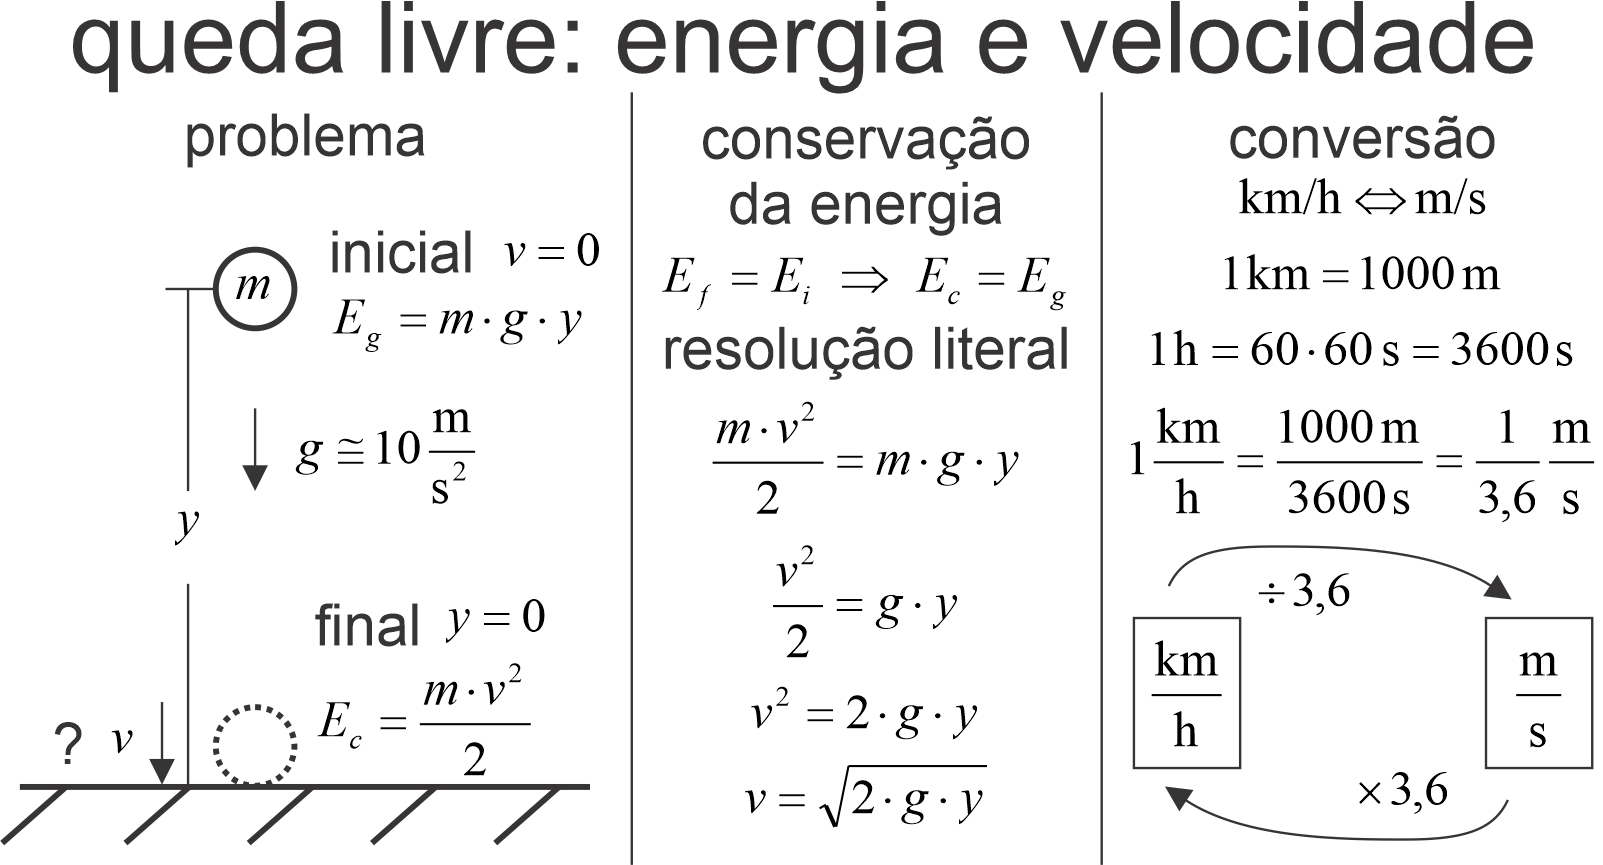
\includegraphics[scale=0.9]{esquema-queda-livre}
\par\end{centering}
\caption{Esquema para dedução da velocidade de queda livre, baseada na conservação
da energia, para implantar aplicações em código.}\label{fig:esquema-queda-livre}
\end{figure}

\begin{figure}[H]
\begin{centering}
\begin{tabular}{ll}
\textbf{expressão} & \textbf{comentário}\tabularnewline
\texttt{\textbf{y = 3000}} & \texttt{\textbf{\% definição da altura de queda livre em metros}}\tabularnewline
\texttt{\textbf{g = 10}} & \texttt{\textbf{\% definição da aceleração da gravidade em m/s\textasciicircum 2}}\tabularnewline
\texttt{\textbf{v = sqrt(2{*}g{*}y)}} & \texttt{\textbf{\% cômputo da velocidade de queda livre em m/s}}\tabularnewline
\texttt{\textbf{km = 1000}} & \texttt{\textbf{\% quilômetro em metros}}\tabularnewline
\texttt{\textbf{h = 60{*}60}} & \texttt{\textbf{\% hora em segundos}}\tabularnewline
\texttt{\textbf{m\_s = km/h}} & \texttt{\textbf{\% fator de conversão km/h em m/s}}\tabularnewline
\texttt{\textbf{km\_h = 1/m\_s}} & \texttt{\textbf{\% fator de conversão m/s em km/h}}\tabularnewline
\texttt{\textbf{v\_m\_s = v}} & \texttt{\textbf{\% velocidade de queda livre em m/s}}\tabularnewline
\texttt{\textbf{v\_km\_h = v {*} km\_h}} & \texttt{\textbf{\% velocidade de queda livre em km/h}}\tabularnewline
\end{tabular}
\par\end{centering}
\caption{Código para execução do cômputo da velocidade de queda livre.}\label{fig:codigo-queda-livre}
\end{figure}

Este exemplo contraria o primeiro axioma que adotamos, ao usar o princípio
da conservação da energia, contrariando a gênese histórica e lógica
do problema. Justificamos este caso, pois nos apegamos ao objetivo
de treinar habilidades de codificação da solução numérica e enfatizamos
que a dedução feita dessa forma “quebra” a gênese histórica do problema
ao lançar mão do princípio de conservação da energia.

Que fique esclarecido que os dois princípios axiomáticos que adotamos
servem de argumentação e justificação da síntese teórica que esboçamos,
mas não devem ser tomados como regras rígidas dessa metodologia. A
resolução literal, o uso de uma ferramenta de computação numérica
como o MathJSLab e o segundo axioma associado à ideia de treinar habilidades
de codificação garantem que este exemplo ainda esteja alinhado à metodologia
proposta.

\section{CONCLUSÃO}

Neste trabalho, nos propomos a dar início a uma aproximação teórica
entre a TAR e a TAHC, com o objetivo de delinear uma metodologia de
Ensino de Física baseada na Resolução Literal de Problemas. Apesar
de apenas esboçarmos essa aproximação teórica sem chegar a uma síntese
definitiva, elencamos diretrizes axiomáticas consistentes da epistemologia
genética e da psicologia do desenvolvimento. Estas sim são evidentes
e definitivas, além de perfeitamente alinhadas à metodologia que propomos.

Propomos uma fundamentação teórica inovadora para o Pensamento Computacional,
transcendendo visões meramente técnicas ao integrá-lo a uma síntese
sociotécnica entre a TAR e a TAHC. Essa abordagem redefine os quatro
pilares clássicos da disciplina não apenas como habilidades cognitivas,
mas como processos de internalização de mediações culturais e construção
de redes sociotécnicas entre humanos e não humanos.

Concluímos fornecendo o recurso didático para realizar ações com a
metodologia que propomos na forma de um software maduro, o MathJSLab,
com disponibilidade livre, possibilidade de desenvolvimento colaborativo,
podendo ser usado pela Web.

Desenvolvimentos futuros do software habilitarão ele a produzir anotações
contendo equações, gráficos, figuras, esquemas, fluxogramas, etc.,
editados de maneira simples no formato Markdown, para que alunos e
professores possam produzir facilmente anotações de qualidade. Já
está sendo trabalhada a adaptação do software para poder ser publicado
também em lojas online de aplicativos.

\printbibliography

\end{document}
